\documentclass{unitothesis}

% \includeonly{}

% Packages for TikZ NNs
\usepackage{listofitems} % for \readlist to create arrays
\usetikzlibrary{arrows.meta} % for arrow size
\usepackage[outline]{contour} % glow around text
\contourlength{1.4pt}

% Colors for TikZ NNs
\colorlet{myred}{red!80!black}
\colorlet{myblue}{blue!80!black}
\colorlet{mygreen}{green!60!black}
\colorlet{myorange}{orange!70!red!60!black}
\colorlet{mydarkred}{red!30!black}
\colorlet{mydarkblue}{blue!40!black}
\colorlet{mydarkgreen}{green!30!black}

% Styles for TikZ NNs
\tikzset{
    >=latex, % for default LaTeX arrow head
    node/.style={thick,circle,draw=myblue,minimum size=22,inner sep=0.5,outer sep=0.6},
    node bias/.style={node,black!90,draw=black,fill=black!25},
    node in/.style={node,green!20!black,draw=mygreen!30!black,fill=mygreen!25},
    node hidden/.style={node,blue!20!black,draw=myblue!30!black,fill=myblue!20},
    node out/.style={node,red!20!black,draw=myred!30!black,fill=myred!20},
    connect/.style={thick,mydarkblue}, %,line cap=round
    connect arrow/.style={-{Latex[length=4,width=3.5]},thick,mydarkblue,shorten <=0.5,shorten >=1},
    node 0/.style={node bias}, % node styles, numbered for easy mapping with \nstyle
    node 1/.style={node in},
    node 2/.style={node hidden},
    node 3/.style={node out}
}
\def\nstyle{int(\curr<\Nnodlen?min(2,\curr):3)} % map layer number onto 1, 2, or 3

% Reset section counter after new part
\usepackage{chngcntr}
\counterwithin*{section}{part}

% Useful commands for this project
\newcommand{\J}{\mathcal{J}}
\newcommand{\mono}[1]{\texttt{#1}}
\newcommand{\mfnet}{\mono{mfnet}\xspace}
\newcommand{\pytorch}{\mono{PyTorch}\xspace}
\newcommand{\shape}[2]{$#1\times #2$}
\newcommand{\wrt}{with respect to\xspace}
\newcommand{\nin}{n_\text{in}}
\newcommand{\nout}{n_\text{out}}

% Acronyms
\acrodef{FFCNN}{Feedforward Fully Connected Neural Network}
\acrodef{MSE}{Mean Squared Error}
\acrodef{CE}{Cross Entropy}
\acrodef{NN}{Neural Network}
\acrodef{GD}{Gradient Descent}
\acrodef{SGD}{Stochastic Gradient Descent}

\DeclareSIUnit\pixel{px}

\author{Francesco Marchisotti}
\title{\centering\mfnet \sc-- A simple\\[0.5em] Machine Learning Library}
\aayear{2024/2025}

\begin{supervisors}
   \supervisor{}{}{\sc Matteo Osella}
\end{supervisors}

\begin{document}

\maketitlepage
\thispagestyle{empty}
\subsection*{\centering Abstract}
Modern machine learning libraries such as \pytorch and \mono{TensorFlow} are widely used in both academia and industry. They are highly optimized, feature-rich, and provide extensive support for various machine learning tasks. In addition to their extensive features, these libraries are designed to efficiently leverage modern GPUs to significantly speed up training and inference for large-scale machine learning models.

To gain a deeper understanding of the workings of such libraries, \mfnet was developed as a simplified neural network library from scratch. The main objective was to implement a functional framework, focusing on the core concept of backpropagation.

The effectiveness of the library was validated by analyzing learning curves on two benchmark tasks: regression and classification. The results demonstrate that \mfnet successfully learns and generalizes, confirming the correctness of its implementation.

\newpage

{\hypersetup{linkcolor=black}\tableofcontents}

% \addcontentsline{toc}{section}{Signal Flow in \aclp*{NN}}
\section*{Signal Flow in \aclp*{NN}}

A \ac{FFCNN} is a \ac{NN} architecture where each neuron in one layer is connected to every neuron in the subsequent layer. A \ac{FFCNN} learns by iteratively performing two main steps: the forward pass and the backward pass.

\begin{figure}[h]
    \centering
    % NEURAL NETWORK with coefficients, arrows
    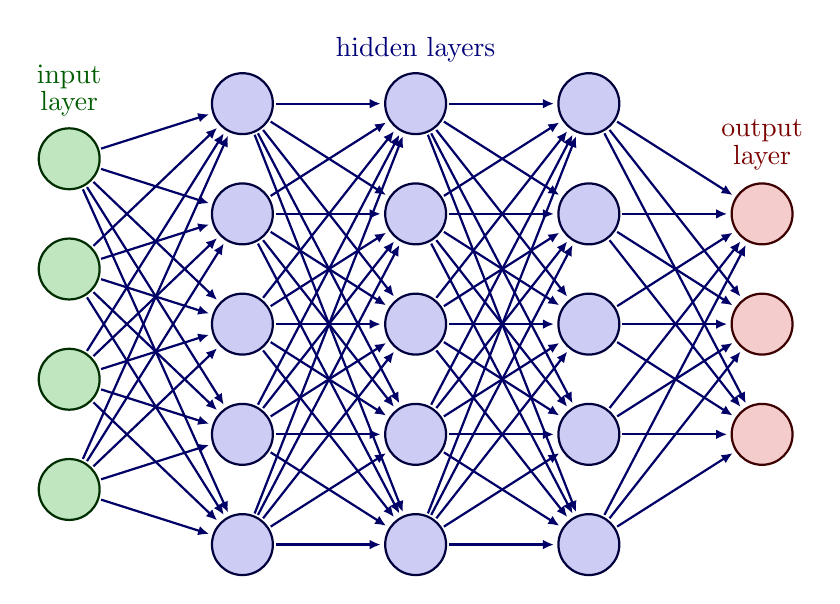
\begin{tikzpicture}[x=2.2cm,y=1.4cm]
    \readlist\Nnod{4,5,5,5,3} % array of number of nodes per layer

    \foreachitem \N \in \Nnod{ % loop over layers
        \edef\curr{\Ncnt} % alias of index of current layer
        \pgfmathsetmacro\prev{int(\Ncnt-1)} % number of previous layer
        \foreach \i [evaluate={\y=\N/2-\i; \x=\curr; \n=\nstyle;}] in {1,...,\N}{ % loop over nodes

        % NODES
        \node[node \n] (N\curr-\i) at (\x,\y) {};

        % CONNECTIONS
        \ifnum\curr>1 % connect to previous layer
            \foreach \j in {1,...,\Nnod[\prev]}{ % loop over nodes in previous layer
                \draw[connect arrow] (N\prev-\j) -- (N\curr-\i); % connect arrows directly
            }
        \fi

        }

    }

    % LABELS
    \node[above=0.3,align=center,mygreen!60!black] at (N1-1.90) {input\\[-0.2em]layer};
    \node[above=0.1,align=center,myblue!60!black] at (N3-1.90) {hidden layers};
    \node[above=0.8,align=center,myred!60!black] at (N\Nnodlen-1.90) {output\\[-0.2em]layer};

    \end{tikzpicture}
    \caption{\Iac{FFCNN}.}
    \label{fig:fcnn}
\end{figure}

\paragraph{Forward pass} The input data is propagated through the network, layer by layer, to produce an output prediction. This prediction is then compared to the true target values using a loss function, which quantifies the prediction error.

\paragraph{Backward pass} The network uses the computed loss to adjust its internal parameters. This is done by propagating the error backward through the network and updating the weights to minimize the loss. The process of forward and backward passes is repeated for multiple iterations, gradually improving the model's performance. This step is the heart of the learning process, as it allows the network to learn from its mistakes and improve its predictions over time.


\part{Implementation of \mfnet}

This first part describes the implementation details of the \mfnet library.

All the code for this project is available on \href{https://www.github.com/marchfra/mfnet}{GitHub}.

\part{Implementation of \texttt{mfnet}}

\section{Basic Data Structure}

The fundamental data structure in \texttt{mfnet} is the Tensor. In this context, a Tensor is simply a \texttt{numpy}
array with a fixed data type of \texttt{numpy.float64}. 

Tensors are used throughout \texttt{mfnet} to represent inputs, outputs, intermediate activations, weights, and
gradients within the neural network.

\section{Backpropagation} \label{sec:backprop}
Before diving into the details of the implementation of \texttt{mfnet}, it's necessary to understand the algorithm at the core of the learning process: backpropagation.

The algorithm is more easily understandable using the indices notation, but in order to implement it in code, we need to express it in matrix form, so both formulations will be shown.

{\color{red}
We define $m$ to be the number of samples, $n^{[l]}$ the number of neurons in layer $l$, $a_j^{[l]}$ the activation of neuron $j$ in layer $l$ (with $a_1^{[l]} = 1$), and $W_{jk}^{[l]}$ the weight connecting neuron $k$ in layer $l-1$ to neuron $j$ in layer $l$ (with $W_{j1}^{[l]} = b_j^{[l]}$ and $W_{1k}^{[l]} = \delta_{1k}$).
}

The goal of the backpropagation algorithm is to compute the derivative of the loss with respect to each weight in the network using the chain rule.

\paragraph{Indices notation}
The flow of information through layer $l$ is given by:
\begin{gather*}
    z_j^{[l]} = \sum_{k=1}^{n^{[l-1]}} W_{jk}^{[l]} a_k^{[l-1]} \\
    a_j^{[l]} = g\left(z_j^{[l]}\right)
\end{gather*}

The derivative of the loss $\J$ with respect to the weights $W_{jk}^{[l]}$ is computed as:
\begin{align*}
    \pdv{\J}{W_{jk}^{[l]}} &= \pdv{\J}{z_j^{[l]}} \pdv{z_j^{[l]}}{W_{jk}^{[l]}}\\
    &= \Delta_j^{[l]} \pdv{z_j^{[l]}}{W_{jk}^{[l]}} = \Delta_j^{[l]} a_k^{[l-1]}
\end{align*}

Now, $\Delta_j^{[l]}$ can be expressed in function of $\Delta_j^{[l + 1]}$:
\begin{align*}
    \Delta_j^{[l]} = \pdv{\J}{z_j^{[l]}} &= \pdv{\J}{a_j^{[l]}} \pdv{a_j^{[l]}}{z_j^{[l]}}\\
    &= \left( \sum_{i=1}^{n^{[l + 1]}} \pdv{\J}{z_i^{[l+1]}} \pdv{z_i^{[l+1]}}{a_j^{[l]}} \right) \pdv{a_j^{[l]}}{z_j^{[l]}}\\
    &= \left( \sum_{i=1}^{n^{[l + 1]}} \Delta_i^{[l+1]} W_{ij}^{[l+1]} \right) g'\left(z_j^{[l]}\right)
\end{align*}

The procedure can be iterated until the last layer $L$ is reached:
\begin{align*}
    \Delta_j^{[L]} = \pdv{\J}{z_j^{[L]}} = \pdv{\J}{a_j^{[L]}} \pdv{a_j^{[L]}}{z_j^{[L]}} = \pdv{\J}{\hat{y_j}} f'\left(z_j^{[L]}\right)
\end{align*}

This last term can be computed after the forward pass is completed. By iteration, every $\Delta_j^{[l]}$ can be computed, and thus every $\pdv{\J}{W_{jk}^{[l]}}$.

\paragraph{Matrix notation} Matrix notation can be easily derived from the indices notation, being careful with the order of the products and with placing the transposed.

The flow of information through layer $l$ is given by:
\begin{gather*}
    Z^{[l]} = W^{[l]} A^{[l-1]}\\
    A^{[l]} = g\left(Z^{[l]}\right)
\end{gather*}

The derivative of the loss $\J$ with respect to the weights $W^{[l]}$ is computed as:
\begin{equation*}
    \pdv{\J}{W^{[l]}} = \pdv{\J}{Z^{[l]}} \pdv{Z^{[l]}}{W^{[l]}} = \Delta^{[l]} A^{[l-1]T}
\end{equation*}

Now, $\Delta^{[l]}$ can be expressed in function of $\Delta^{[l + 1]}$:
\begin{align*}
    \Delta^{[l]} = \pdv{\J}{Z^{[l]}} &= \pdv{\J}{A^{[l]}} \odot \pdv{A^{[l]}}{Z^{[l]}}\\
    &= \left(\pdv{Z^{[l+1]}}{A^{[l]}} \pdv{\J}{Z^{[l+1]}} \right) \odot \pdv{A^{[l]}}{Z^{[l]}}\\
    &= \left(W^{[l+1]T} \Delta^{[l+1]} \right) \odot g'\left(Z^{[l]}\right)
\end{align*}
where $\odot$ denotes the element-wise (Hadamard) product.

The procedure can be iterated until the last layer $L$ is reached:
\begin{align*}
    \Delta^{[L]} = \pdv{\J}{Z^{[L]}} = \pdv{\J}{A^{[L]}} \odot \pdv{A^{[L]}}{Z^{[L]}} = \pdv{\J}{\hat{Y}} \odot f'\left(Z^{[L]}\right)
\end{align*}

This last term can be computed after the forward pass is completed. By iteration, every $\Delta^{[l]}$ can be computed, and thus every $\pdv{\J}{W^{[l]}}$.

\section{Layer}

In \texttt{mfnet}, a layer is a fundamental building block of the neural network. Each layer consists of a set of neurons, and it performs a specific transformation on the input data. The two main types of layers implemented in \texttt{mfnet} are Linear layers and Activation layers.

% \begin{itemize}
%     \item \textbf{Linear Layer:} This layer applies a linear transformation to the input data, represented by the equation $y = Ax + b$, where $A$ is the weight matrix, $x$ is the input vector, $b$ is the bias vector, and $y$ is the output vector.
%     \item \textbf{Activation Layer:} This layer applies a non-linear activation function to the output of the linear layer. Common activation functions include ReLU (Rectified Linear Unit), Sigmoid, and Tanh.
% \end{itemize}

Layers are stacked together to form a complete neural network, with the output of one layer serving as the input to the next layer.  Each layer is responsible for maintaining its own parameters and computing gradients during the backpropagation process.

Each of the layers in \texttt{mfnet} expects the input to be in the form of a matrix with shape $(n_{\text{features}} + 1, n_{\text{samples}})$, where $n_{\text{features}}$ is the number of input features and $n_{\text{samples}}$ is the number of input samples. The first row of this matrix is reserved for a bias term, which is always set to 1.

\subsection{Linear Layer}
\subsubsection{Forward pass}
The Linear layer in \texttt{mfnet} applies a linear transformation to the input data, performing a change in dimensionality from $n_{\text{in\_features}}$ to $n_{\text{out\_features}}$. Mathematically, this can be represented as:
\begin{equation}
    y = b + Wx
\end{equation}

where:
\begin{itemize}
    \item $x$ is the $(n_{\text{in\_features}}, 1)$ input vector,
    \item $W$ is the $(n_{\text{out\_features}}, n_{\text{in\_features}})$ weight matrix,
    \item $b$ is the $(n_{\text{out\_features}}, 1)$ bias vector, and
    \item $y$ is the $(n_{\text{out\_features}}, 1)$ output vector.
\end{itemize}

\paragraph{Implementation Details} The actual implementation is a bit different: the first key difference is that the bias term is absorbed inside the weights matrix, and the input vector is augmented with an additional constant value of 1. The layer expects this ``bias feature'' to be already present in the input data, and propagates it to the next layer by adding a row of $\begin{pmatrix}1 & 0 \cdots 0\end{pmatrix}$ to the weights matrix. This allows us to rewrite the equation as:
\begin{equation}
    \begin{pmatrix} 1 \\ y \end{pmatrix} = \begin{pmatrix} 1 & 0 \cdots 0 \\ b & W \end{pmatrix} \begin{pmatrix} 1 \\ x \end{pmatrix}
\end{equation}

The second key difference is that, instead of feeding one data point at a time to the network and heavily relying on inefficient for loops, we can feed a batch of data points at once, and leverage efficient matrix operations. This means that the input $x$ is actually a matrix $X$ where each column represents a different data point, and the output $y$ is also a matrix $Y$ where each column corresponds to the output for each input data point. The equation then becomes:
\begin{equation}
    \begin{pmatrix} 1 \cdots 1 \\ Y \end{pmatrix} = \begin{pmatrix} 1 & 0 \cdots 0 \\ b & W \end{pmatrix} \begin{pmatrix} 1 \cdots 1 \\ X \end{pmatrix}
\end{equation}

Switching to standard backpropagation notation, we can summarize the forward pass of a Linear layer as:
\begin{equation}
    Z^{[l]} = W^{[l]} A^{[l - 1]}
\end{equation}
where:
\begin{itemize}
    \item $A^{[l - 1]}$ is the input of the Linear layer $l$, with $A^{[0]}$ being the input data (shape $(n_{\text{features}} + 1, n_{\text{samples}})$),
    \item $W^{[l]}$ is the weights matrix of the Linear layer $l$ (shape $(n_{\text{out\_features}} + 1,\\ n_{\text{in\_features}} + 1)$), and
    \item $Z^{[l]}$ is the output of the Linear layer $l$ (shape $(n_{\text{out\_features}} + 1, n_{\text{samples}})$).
\end{itemize}
All these Tensors already include all the necessary additions to correctly handle the bias.

The Linear layer forward method also stores its input $A^{[l - 1]}$ for use in the backward pass.

\subsubsection{Backward pass}
The Linear layer's responsibility is to compute the gradients of the loss with respect to its weights during the backward pass.

\section{Loss}
The final ingredient in the training of a neural network is the loss function. This function measures the error between the predicted output of the network and the true target values. The goal of training is to minimize this loss function by adjusting the weights of the network through backpropagation.

Also, as seen in Section \ref{sec:backprop}, the derivative of the loss with respect to the output of the network is needed to start the backpropagation process.

\texttt{mfnet} implements two of the most important loss functions: Mean Squared Error (MSE), used mainly in regression tasks, and Cross Entropy (CE), used in classification tasks.

\subsection{Mean Squared Error (MSE)}
The Mean Squared Error loss function is defined as:
\begin{equation}
    \J(\hat{y}, y) = \frac{1}{m} \sum_{i=1}^{m} \norm{\hat{y}_i - y_i}^2 = \frac{1}{m} \sum_{i=1}^{m} \sum_{j=1}^{n_\text{feat}} (\hat{y}_{ij} - y_{ij})^2
\end{equation}
where $\hat{y}_i$ is the vector of predicted values for the $i$-th sample, $y_i$ is the vector of true target values for the $i$-th sample and $m$ is the number of samples. It represents the square modulus of the error vector, averaged over all samples.

The gradient matrix of the loss with respect to the output of the network is given by:
\begin{equation}
    \pdv{\J}{\hat{y}} = \frac{2}{m} (\hat{y} - y)
\end{equation}

\section{\acl*{NN}, Optimizer and Dataloader}
In this section we describe the implementation of more high-level objects that can be built using the building blocks described in the previous sections.

\subsection{\acl*{NN}}
A \acl{NN} is made up of a sequence of layers, each one transforming the input tensor into an output tensor, and each one feeding into the next.

As far as coding is concerned, it is a very simple object, and only defines three methods: forward, backward and a method that yields an iterator on all the layers' parameters.

The forward method simply calls the forward method of each layer in sequence, passing the output of one layer as input to the next one.

The backward method does the opposite: it calls the backward method of each layer in reverse order, passing the gradient of the loss with respect to the input of each layer as input to the previous layer.

\subsection{Optimizer}
The optimizer is responsible for updating the parameters of the \acl{NN} during training.

The most basic optimizer is \ac{GD}, which updates the parameters according to the rule:
\begin{equation}
    W^{[l]} \gets W^{[l]} - \eta \pdv{\J}{W^{[l]}}
\end{equation}
where $\eta$ is the learning rate.

This algorithm in this form suffers from many problems, such as having a big computational overhead and not being able to escape local minima. A more robust version is \ac{SGD}, which updates the parameters using a mini-batch (see \cref{sec:dataloader}) of data instead of the whole dataset. This introduces some noise in the updates, which can help the optimizer to escape local minima.

\paragraph{Implementation details} When training a full \ac{NN} using ReLUs as activation functions, there was often an overflow problem. To help mitigate this, the \mono{Optimizer} class implements gradient clipping, which prevents the gradients from becoming too large by clipping the norm of the gradient tensor to a maximum value provided by the user.

\subsection{Dataloader} \label{sec:dataloader}
The dataloader is responsible for loading the data in mini-batches and shuffling it at the beginning of each epoch. This is important for \ac{SGD} to work properly, as it helps to reduce the correlation between consecutive mini-batches and improves the convergence of the optimizer.

\paragraph{Implementation details} In addition to creating the mini-batches, the\\\mono{DataLoader} class is also responsible for transforming the data, which is usually stored in a \shape{m}{n_\text{features}} matrix (the design matrix), into a format compatible with the \mfnet library: first, the design matrix is transposed, so that each column represents a data sample and each row represents a feature; then, the bias feature is prepended to the input data as a row of 1s. The same transformations are applied to the target data.

\paragraph{Example}
For a complete step-by-step example of how the learning process works, please refer to \cref{sec:example}.

\section{Training utilities} \label{sec:training-utilities}

The most useful function provided by the \mono{trainutils.py} module is\\\mono{train\_test\_split}. This function takes as input two tensors (input data and target data) and splits them into training and test sets.

Other notable functions include \mono{normalize\_features} and\\\mono{denormalize\_features}, which are used to normalize and denormalize the input and target features, respectively; \mono{one\_hot\_encode} and \mono{one\_hot\_decode}, which are used to convert categorical labels into one-hot encoded vectors and vice versa; and \mono{accuracy}, which computes the accuracy of predictions for classification tasks, i.e., the number of correct predictions divided by the total number of samples.

\section{Train}

The \mono{train.py} module implements three convenience functions for training and testing neural networks: \mono{train}, \mono{train\_test\_regression} and\\\mono{train\_test\_classification}.

All three of these functions implement the basic training cycle: for each epoch, iterate over the training dataset in batches, perform a forward pass, compute the loss, perform a backward pass to compute gradients, clip the gradients if the user specified a maximum norm, and update the model parameters using the optimizer. At the end of each epoch, the loss is averaged over all batches and appended to a list, which is returned at the end of training.

While the \mono{train} function stops there, the other two functions also evaluate the model on a test dataset at the end of each epoch, and return both the training and test losses. \mono{train\_test\_classification} also computes the accuracy on the test set.




\part{Comparison with \pytorch}

In order to check that all the implementation of \mfnet is correct, two simple tasks have been performed and compared with \pytorch: a regression task on the California Housing dataset and a classification task on the MNIST dataset.

The two tasks have been implemented as closely as possible in both libraries, using the same architecture, loss function and optimizer. Training hyperparameters such as learning rate and batch size were different between the two frameworks, as using the same values for both resulted in a more unstable training for one of the two libraries.

Note that the goal of the project was not to outperform \pytorch, but rather to compare the training process of \mfnet with that of a production machine learning framework and check that the overall behavior is consistent with the expectations of a functioning library.

The code for the comparison can be found on \href{https://github.com/marchfra/interface}{GitHub}.

\part{Comparison with \pytorch}

In order to check that all the implementation of \mfnet is correct, two simple tasks have been performed and compared with \pytorch: a regression task on the California Housing dataset and a classification task on the MNIST dataset.

The two tasks have been implemented as closely as possible in both libraries, using the same architecture, loss function and optimizer. Training hyperparameters such as learning rate and batch size varied slightly between the two frameworks, as using the same values for both resulted in a worse training for one of the two libraries.

The code for the comparison can be found on \href{git@github.com:marchfra/interface.git}{GitHub}.

\section{Regression on California Housing}

After the data was loaded and split in training and test sets, feature normalisation was performed on the training set. Using the statistics learned from the training set, the test set was normalised in the same way.

The training hyperparameters used for both libraries are shown in the \cref{tab:regr_hyperparams}.
\begin{table}[hb]
\centering
\begin{tabular}{|c|c|c|}
    \hline
    Hyperparameter & \mfnet & \pytorch \\
    \hline
    Number of Epochs & 500 & 500 \\
    Learning Rate $\eta$ & 0.001 & 0.001 \\
    Batch Size & 1024 & 1024 \\
    \hline
\end{tabular}
\caption{Training hyperparameters for regression task.}
\label{tab:regr_hyperparams}
\end{table}

For each libraries, three models were trained and compared:
\begin{enumerate}
    \item a naive mean predictor that always predicts the mean value of the training set;
    \item a linear regression model;
    \item a neural network with one hidden layer of 512 neurons and ReLU activation functions. For \mfnet only, maximum gradient norm was set to 5 in order to prevent overflow errors.
\end{enumerate}

The learning curves for both libraries are shown in \cref{fig:regr_mfnet,fig:regr_pytorch}.

\begin{figure}
    \centering
    \includegraphics[width=0.75\linewidth]{Images/mfnet_regr_mserror_500_0.001_1024.png}
    \caption{Learning curves for regression task on California Housing dataset using \mfnet.}
    \label{fig:regr_mfnet}
\end{figure}

\begin{figure}
    \centering
    \includegraphics[width=0.75\linewidth]{Images/pytorch_regr_mserror_500_0.001_1024.png}
    \caption{Learning curves for regression task on California Housing dataset using \pytorch.}
    \label{fig:regr_pytorch}
\end{figure}

\section{Classification on MNIST}

After loading the data (already split in training and test sets), the pixel values were normalized to the range [0, 1]. \mfnet also required the data to be transformed in such a way that the library would be able to understand.

The training hyperparameters used for both libraries are shown in the \cref{tab:class_hyperparams}.
\begin{table}[ht]
\centering
\begin{tabular}{|c|c|c|}
    \hline
    Hyperparameter & \mfnet & \pytorch \\
    \hline
    Number of Epochs & 100 & 100 \\
    Learning Rate $\eta$ & 0.001 & 0.01 \\
    Batch Size & 1024 & 128 \\
    \hline
\end{tabular}
\caption{Training hyperparameters for classification task.}
\label{tab:class_hyperparams}
\end{table}

For each library, two models were trained and compared:
\begin{enumerate}
    \item a linear classification model;
    \item a neural network with one hidden layer of 512 neurons and ReLU activation functions. For \mfnet only, maximum gradient norm was set to 5 in order to prevent overflow errors.
\end{enumerate}

The learning curves and test accuracies for both libraries are shown in \cref{fig:class_mfnet,fig:class_pytorch}.

\begin{figure}[ht]
    \centering
    \includegraphics[width=0.75\linewidth]{Images/mfnet_class_loss_acc_100_0.001_1024.png}
    \caption{Learning curves for classification task on MNIST dataset using \mfnet.}
    \label{fig:class_mfnet}
\end{figure}

\begin{figure}[ht]
    \centering
    \includegraphics[width=0.75\linewidth]{Images/pytorch_class_loss_acc_100_0.01_128.png}
    \caption{Learning curves for classification task on MNIST dataset using \pytorch.}
    \label{fig:class_pytorch}
\end{figure}

The accuracy achieved by \pytorch is significantly lower than the one achieved by \mfnet, so the confusion matrices for both libraries are computed and shown in \cref{fig:conf_mfnet,fig:conf_pytorch}. The figures clearly show that, while \mfnet is able to correctly classify almost all the digits, \pytorch struggles with most of them (particularly the digits 0 and 8).

\begin{figure}[ht]
    \centering
    \includegraphics[width=0.85\linewidth]{Images/mfnet_class_conf_matrix_100_0.001_1024.png}
    \caption{Confusion matrix for classification task on MNIST dataset using \mfnet.}
    \label{fig:conf_mfnet}
\end{figure}

\begin{figure}[ht]
    \centering
    \includegraphics[width=0.85\linewidth]{Images/pytorch_class_conf_matrix_100_0.01_128.png}
    \caption{Confusion matrix for classification task on MNIST dataset using \pytorch.}
    \label{fig:conf_pytorch}
\end{figure}

\section*{A note on execution times}
It is interesting to note the execution times of the training loops for both libraries, shown in \cref{tab:regr_times,tab:class_times}. All training was done on a MacBook Pro 2019 with a 2.3 GHz Quad-Core Intel Core i7 processor, as \mfnet is not optimized to run on GPUs.

\begin{table}[ht]
\centering
\begin{tabular}{|c|c|c|}
    \hline
    Model & \mfnet & \pytorch \\
    \hline
    Naive Mean Predictor & $\SI{0.0}{\s}$ & $\SI{0.0}{\s}$ \\
    Linear Regression & $\SI{1.1}{\s}$ & $\SI{58.2}{\s}$ \\
    Neural Network & $\SI{238.3}{\s}$ & $\SI{122.1}{\s}$ \\
    \hline
\end{tabular}
\caption{Execution times for regression training loops.}
\label{tab:regr_times}
\end{table}

\begin{table}[ht]
\centering
\begin{tabular}{|c|c|c|}
    \hline
    Model & \mfnet & \pytorch \\
    \hline
    Linear Classification & $\SI{145.5}{\s}$ & $\SI{700.8}{\s}$ \\
    Neural Network & $\SI{401.7}{\s}$ & $\SI{801.4}{\s}$ \\
    \hline
\end{tabular}
\caption{Execution times for classification training loops.}
\label{tab:class_times}
\end{table}

While \mfnet is almost always significantly faster that \pytorch, \pytorch's times are more consistent between models. This is probably due to the fact that \pytorch is a highly optimised library, while \mfnet is a simple implementation: the advantage of \mfnet likely comes from its simplicity, while the more consistent times of \pytorch show that its a more mature library, although with room for improvement.

The models trained were also quite simple, with the \aclp{NN} having at most one hidden layer. This means that the execution times may not fully represent the capabilities of each library when dealing with more complex architectures.


\appendix

\newpage
\section{Step-by-step example of an epoch} \label{sec:example}
To better understand how the bias is handled throughout \mfnet, it's helpful to consider a practical example: we'll walk through a forward/backward cycle of a small network with two hidden layers and all the activation functions set to the identity.

\begin{figure}[h]
    \centering
    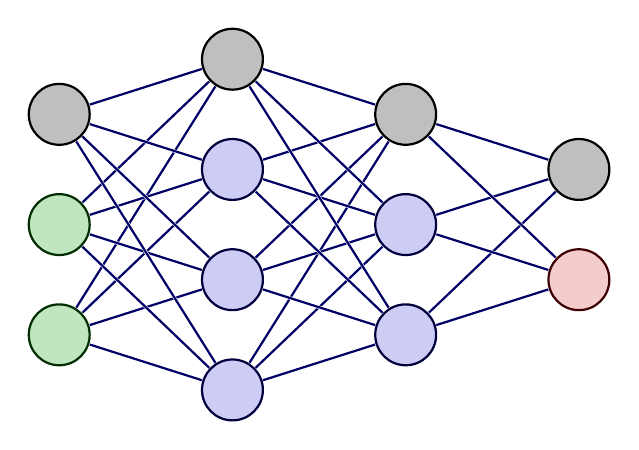
\begin{tikzpicture}[x=2.2cm,y=1.4cm]
        \readlist\Nnod{3,4,3,2} % array of number of nodes per layer

        \foreachitem \N \in \Nnod{ % loop over layers
            \def\curr{\Ncnt} % alias of index of current layer
            \pgfmathsetmacro\prev{int(\Ncnt-1)} % number of previous layer
            \foreach \i [evaluate={\y=\N/2-\i; \x=\curr; \n=\nstyle;}] in {1,...,\N}{ % loop over nodes

                % NODES
                \ifnum\i=1
                    \node[node 0] (N\curr-\i) at (\x,\y) {};
                \else
                    \node[node \n] (N\curr-\i) at (\x,\y) {};
                \fi

                % CONNECTIONS
                \ifnum\curr>1 % connect to previous layer
                    \foreach \j in {1,...,\Nnod[\prev]}{ % loop over nodes in previous layer
                        \draw[connect,white,line width=1.2] (N\prev-\j) -- (N\curr-\i);
                        \draw[connect] (N\prev-\j) -- (N\curr-\i);
                    }
                \fi

            }
        }
    \end{tikzpicture}
    \caption{A small \acl{NN} with two hidden layers. The gray neurons represent the bias features.}
    \label{fig:small-nn}
\end{figure}

Let's pick an input $X$ and target $Y$:
\begin{equation*}
    X = \mqty[
        1 & 2 \\
        1 & 2 \\
        2 & 2 \\
        2 & 3
    ], \quad
    Y = \mqty[1 \\ 1 \\ 2 \\ 2]
\end{equation*}

This is a small dataset of four samples with two input features and one target feature.

First, the \mono{DataLoader} transposes the data and prepends the bias feature:
\begin{equation*}
    A^{[0]} = \tilde{X} = \mqty[
        \color{red} 1 & \color{red} 1 & \color{red} 1 & \color{red} 1 \\
        1 & 1 & 2 & 2 \\
        2 & 2 & 2 & 3
    ], \quad \tilde{Y} = \mqty[
        \color{red} 1 & \color{red} 1 & \color{red} 1 & \color{red} 1 \\
        1 & 1 & 2 & 2
    ]
\end{equation*}

\newpage
\subsection{Forward pass}
Now the \mono{forward} method of the \mono{NeuralNetwork} is called with input data $A^{[0]}$.

\paragraph{Layer 1 (Linear)} The first layer is a Linear layer with 2 input features (plus bias) and 3 output features (plus bias). Suppose the weights matrix $W^{[1]}$ is:
\begin{equation*}
    W^{[1]} = \mqty[
        \color{red} 1 & \color{red} 0 & \color{red} 0 \\
        0 & 0 & 1 \\
        0 & 1 & 1 \\
        1 & 0 & 0
    ]
\end{equation*}

Then, the output of the layer is:
\begin{equation*}
    Z^{[1]} = W^{[1]} A^{[0]} = \mqty[
        \color{red} 1 & \color{red} 1 & \color{red} 1 & \color{red} 1 \\
        2 & 3 & 2 & 3 \\
        3 & 4 & 4 & 5 \\
        2 & 2 & 3 & 3
    ]
\end{equation*}

\paragraph{Layer 1 (Activation)} The activation function is applied element-wise, skipping the first row:
\begin{equation*}
    A^{[1]} = \mqty[
        \mqty{\color{red} 1 & \color{red} 1 & \color{red} 1 & \color{red} 1} \\
        g(Z^{[1]}[1\hspace{-0.6ex}:])
    ] = \mqty[
        \color{red} 1 & \color{red} 1 & \color{red} 1 & \color{red} 1 \\
        2 & 3 & 2 & 3 \\
        3 & 4 & 4 & 5 \\
        2 & 2 & 3 & 3
    ]
\end{equation*}

\paragraph{Layer 2 (Linear)} The second layer is a Linear layer with 3 input features (plus bias) and 2 output features (plus bias). Suppose the weights matrix $W^{[2]}$ is:
\begin{equation*}
    W^{[2]} = \mqty[
        \color{red} 1 & \color{red} 0 & \color{red} 0 & \color{red} 0\\
        1 & 1 & 0 & 1\\
        -1 & 1 & 2 & -2
    ]
\end{equation*}

Then, the output of the layer is:
\begin{equation*}
    Z^{[2]} = W^{[2]} A^{[1]} = \mqty[
        \color{red} 1 & \color{red} 1 & \color{red} 1 & \color{red} 1 \\
        5 & 6 & 6 & 7 \\
        3 & 6 & 3 & 6
    ]
\end{equation*}

\paragraph{Layer 2 (Activation)} The activation function is applied element-wise, skipping the first row:
\begin{equation*}
    A^{[2]} = \mqty[
        \mqty{\color{red} 1 & \color{red} 1 & \color{red} 1 & \color{red} 1} \\
        g(Z^{[2]}[1\hspace{-0.6ex}:])
    ] = \mqty[
        \color{red} 1 & \color{red} 1 & \color{red} 1 & \color{red} 1 \\
        5 & 6 & 6 & 7 \\
        3 & 6 & 3 & 6
    ]
\end{equation*}

\paragraph{Layer 3 (Linear)} The third layer is a Linear layer with 2 input features (plus bias) and 1 output feature (plus bias). Suppose the weights matrix $W^{[3]}$ is:
\begin{equation*}
    W^{[3]} = \mqty[
        \color{red} 1 & \color{red} 0 & \color{red} 0 \\
        0 & 1 & -1
    ]
\end{equation*}

Then, the output of the layer is:
\begin{equation*}
    Z^{[3]} = W^{[3]} A^{[2]} = \mqty[
        \color{red} 1 & \color{red} 1 & \color{red} 1 & \color{red} 1 \\
        2 & 0 & 3 & 1
    ]
\end{equation*}

\paragraph{Layer 3 (Activation)} The activation function is applied element-wise, skipping the first row:
\begin{equation*}
    \hat{Y} = A^{[3]} = \mqty[
        \mqty{\color{red} 1 & \color{red} 1 & \color{red} 1 & \color{red} 1} \\
        g(Z^{[3]}[1\hspace{-0.6ex}:])
    ] = \mqty[
        \color{red} 1 & \color{red} 1 & \color{red} 1 & \color{red} 1 \\
        2 & 0 & 3 & 1
    ]
\end{equation*}

Now we compute the loss, for instance \ac{MSE}:
\begin{align*}
    \J(\hat{Y}, \tilde{Y}) &= \frac{1}{m} \sum_{i=1}^{m} \norm{\hat{Y}_i - \tilde{Y}_i}^2\\
    &\;\begin{aligned}
        = \frac{1}{4} \left[\right.&(1 - 1)^2 + (1 - 1)^2 + (1 - 1)^2 + (1 - 1)^2 + \\
        &+ (2 - 1)^2 + (0 - 1)^2 + (3 - 2)^2 + (1 - 2)^2\left.\right] = 1
    \end{aligned}
\end{align*}

\subsection{Backward pass}
To start the backward pass, we need to compute the gradient of the loss \wrt the output of the network:
\begin{equation*}
    \frac{\partial \J}{\partial \hat{Y}} = \frac{2}{m} \left(\hat{Y} - \tilde{Y}\right) = \frac{1}{4} \mqty[
        \color{red} 0 & \color{red} 0 & \color{red} 0 & \color{red} 0 \\
        1 & -1 & 1 & -1
    ] = \pdv{\J}{A^{[3]}}
\end{equation*}
This is now the input of the \mono{backward} method of the \mono{NeuralNetwork}.

\paragraph{Layer 3 (Activation)} The backward method of the Activation layer computes the gradient of the loss \wrt its input $Z^{[3]}$. Since the activation function is the identity, its derivative is 1, and we have:
\begin{equation*}
    \Delta^{[3]} = \pdv{\J}{Z^{[3]}} = \pdv{\J}{A^{[3]}} \odot \mqty[
        \mqty{\color{red} 0 & \color{red} 0 & \color{red} 0 & \color{red} 0} \\
        g'(Z^{[3]}[1\hspace{-0.6ex}:])
    ] = \frac{1}{4} \mqty[
        \color{red} 0 & \color{red} 0 & \color{red} 0 & \color{red} 0 \\
        1 & -1 & 1 & -1
    ]
\end{equation*}

\paragraph{Layer 3 (Linear)} The backward method of the Linear layer computes the gradient of the loss \wrt its weights $W^{[3]}$ and its input $A^{[2]}$:
\begin{gather*}
    \pdv{\J}{W^{[3]}} = \Delta^{[3]} A^{[2]T} = \frac{1}{4} \mqty[
        \color{red} 0 & \color{red} 0 & \color{red} 0 \\
        0 & -2 & -6
    ]\\
    \pdv{\J}{A^{[2]}} = W^{[3]T} \Delta^{[3]} = \frac{1}{4} \mqty[
        \color{red} 0 & \color{red} 0 & \color{red} 0 & \color{red} 0 \\
        1 & -1 & 1 & -1 \\
        -1 & 1 & -1 & 1
    ]
\end{gather*}

\paragraph{Layer 2 (Activation)} The backward method of the Activation layer computes the gradient of the loss \wrt its input $Z^{[2]}$. Since the activation function is the identity, its derivative is 1, and we have:
\begin{equation*}
    \Delta^{[2]} = \pdv{\J}{Z^{[2]}} = \pdv{\J}{A^{[2]}} \odot \mqty[
        \mqty{\color{red} 0 & \color{red} 0 & \color{red} 0 & \color{red} 0} \\
        g'(Z^{[2]}[1\hspace{-0.6ex}:])
    ] = \frac{1}{4} \mqty[
        \color{red} 0 & \color{red} 0 & \color{red} 0 & \color{red} 0 \\
        1 & -1 & 1 & -1 \\
        -1 & 1 & -1 & 1
    ]
\end{equation*}

\paragraph{Layer 2 (Linear)} The backward method of the Linear layer computes the gradient of the loss \wrt its weights $W^{[2]}$ and its input $A^{[1]}$:
\begin{gather*}
    \pdv{\J}{W^{[2]}} = \Delta^{[2]} A^{[1]T} = \frac{1}{4} \mqty[
        \color{red} 0 & \color{red} 0 & \color{red} 0 & \color{red} 0 \\
        0 & -2 & -2 & 0 \\
        0 & 2 & 2 & 0 \\
    ]\\
    \pdv{\J}{A^{[1]}} = W^{[2]T} \Delta^{[2]} = \frac{1}{4} \mqty[
        \color{red} 2 & \color{red} -2 & \color{red} 2 & \color{red} -2 \\
        0 & 0 & 0 & 0 \\
        -2 & 2 & -2 & 2 \\
        3 & -3 & 3 & -3 \\
    ]
\end{gather*}

\paragraph{Layer 1 (Activation)} The backward method of the Activation layer computes the gradient of the loss \wrt its input $Z^{[1]}$. Since the activation function is the identity, its derivative is 1, and we have:
\begin{equation*}
    \Delta^{[1]} = \pdv{\J}{Z^{[1]}} = \pdv{\J}{A^{[1]}} \odot \mqty[
        \mqty{\color{red} 0 & \color{red} 0 & \color{red} 0 & \color{red} 0} \\
        g'(Z^{[1]}[1\hspace{-0.6ex}:])
    ] = \frac{1}{4} \mqty[
        \color{red} 0 & \color{red} 0 & \color{red} 0 & \color{red} 0 \\
        0 & 0 & 0 & 0 \\
        -2 & 2 & -2 & 2 \\
        3 & -3 & 3 & -3 \\
    ]
\end{equation*}

\paragraph{Layer 1 (Linear)} The backward method of the Linear layer computes the gradient of the loss \wrt its weights $W^{[1]}$ and its input $A^{[0]}$:
\begin{gather*}
    \pdv{\J}{W^{[1]}} = \Delta^{[1]} A^{[0]T} = \frac{1}{4} \mqty[
        \color{red} 0 & \color{red} 0 & \color{red} 0 \\
        0 & 0 & 0 \\
        0 & 0 & 4 \\
        0 & 0 & -6
    ]\\
    \pdv{\J}{A^{[0]}} = W^{[1]T} \Delta^{[1]} = \frac{1}{4} \mqty[
        \color{red} 3 & \color{red} -3 & \color{red} 3 & \color{red} -3 \\
        1 & -1 & 1 & -1 \\
        -2 & 2 & -2 & 2
    ] \quad \text{(unused)}
\end{gather*}

\subsection{Weight update}

The weights are updated using the \ac{SGD} optimizer:
\begin{equation*}
    W^{[l]} \gets W^{[l]} - \eta \pdv{\J}{W^{[l]}} \\
\end{equation*}

Setting the learning rate $\eta = 4$ for simplicity\footnote{This value is way too high to have any chance of yielding an improvement in the predictions in any practical example.}, we have: 
\begin{gather*}
    W^{[3]} \gets \mqty[
        \color{red} 1 & \color{red} 0 & \color{red} 0 \\
        0 & 1 & -1
    ] - \mqty[
        \color{red} 0 & \color{red} 0 & \color{red} 0 \\
        0 & -2 & -6
    ] = \mqty[
        \color{red} 1 & \color{red} 0 & \color{red} 0 \\
        0 & 3 & 5
    ]\\
    W^{[2]} \gets \mqty[
        \color{red} 1 & \color{red} 0 & \color{red} 0 & \color{red} 0\\
        1 & 1 & 0 & 1\\
        -1 & 1 & 2 & -2
    ] - \mqty[
        \color{red} 0 & \color{red} 0 & \color{red} 0 & \color{red} 0 \\
        0 & -2 & -2 & 0 \\
        0 & 2 & 2 & 0 \\
    ] = \mqty[
        \color{red} 1 & \color{red} 0 & \color{red} 0 & \color{red} 0\\
        1 & 3 & 2 & 1\\
        -1 & -1 & 0 & -2
    ]\\
    W^{[1]} \gets \mqty[
        \color{red} 1 & \color{red} 0 & \color{red} 0 \\
        0 & 0 & 1 \\
        0 & 1 & 1 \\
        1 & 0 & 0
    ] - \mqty[
        \color{red} 0 & \color{red} 0 & \color{red} 0 \\
        0 & 0 & 0 \\
        0 & 0 & 4 \\
        0 & 0 & -6
    ] = \mqty[
        \color{red} 1 & \color{red} 0 & \color{red} 0 \\
        0 & 0 & 1 \\
        0 & 1 & -3 \\
        1 & 0 & 6
    ]
\end{gather*}

Now a new cycle of forward pass/backward pass/weight update can begin.


\end{document}

% Part 2: comparison with pytorch
% \begin{enumerate}
%     \item Regression task
%     \item Classification task
% \end{enumerate}
